\newcommand{\topic}{HIGH FREQUENCY, HALF WAVELENGTH POWER TRANSMISSION}
\newcommand{\name}{RIJO ABRAHAM }
\newcommand{\regno}{13013880}
\newcommand{\guide}{MEERA KHALID}
\newcommand{\guidedesignation}{Assistant Professor}

%-----------------------------------------------------%
\documentclass[12pt,a4paper]{reportmod}
\usepackage{graphicx}
\usepackage{setspace}
\usepackage{tabularx}
\usepackage{amsmath}
\usepackage{tabu}
\usepackage{float}
%-----------------------------------------------------%
%Chapter and Section Font Size and Alignment%
\usepackage{titlesec}
\titleformat{\chapter}[display]
  {\normalfont\centering\large\bfseries}
  {\chaptertitlename\ \thechapter}{0pt}{\Large}
\titleformat{\section}
  {\normalfont\bfseries}
  {\thesection}{1em}{\large}
%-----------------------------------------------------%
%Remove default heading from TOC, LOF & LOT%
\makeatletter
\newcommand*{\toccontents}{\@starttoc{toc}}
\newcommand*{\lofcontents}{\@starttoc{lof}}
\newcommand*{\lotcontents}{\@starttoc{lot}}
\makeatother
%-----------------------------------------------------%
%Font Sizes%
\makeatletter
\renewcommand\normalsize{\@setfontsize\normalsize{12pt}{18}}
\renewcommand\large{\@setfontsize\large{14pt}{16.8}}
\renewcommand\Large{\@setfontsize\Large{16pt}{19.2}}
\renewcommand\LARGE{\@setfontsize\LARGE{18pt}{21.6}}
\renewcommand\huge{\@setfontsize\huge{20pt}{24}}
\makeatother
%-----------------------------------------------------%
%Justication%
\tolerance=1
\emergencystretch=\maxdimen
\hyphenpenalty=10000
\hbadness=10000
%-----------------------------------------------------%
%Margins%
\usepackage[left=1.5 in,right=1.25 in,top=1 in,bottom=1.25 in]{geometry} 
%-----------------------------------------------------%
%Font%
\usepackage[T1]{fontenc}
\usepackage[utf8]{inputenc}
\usepackage{mathptmx}
%-----------------------------------------------------%
%Header and Footer%
\usepackage{fancyhdr}
\pagestyle{fancy}
\fancyhf{}
\rhead{\topic}
\lfoot{RIT, KOTTAYAM}
\cfoot{\thepage}
\rfoot{EEE DEPARTMENT}
\renewcommand{\headrulewidth}{0.4pt}% Default \headrulewidth is 0.4pt
\renewcommand{\footrulewidth}{0.4pt}% Default \footrulewidth is 0pt
\makeatletter
\let\ps@plain\ps@fancy% Include header and footer for plain pages
\makeatother
%-----------------------------------------------------%

%Main%
\begin{document}
\thispagestyle{empty}%Turn off header and footer
\pagenumbering{gobble}%Exclude from page numbering
\newgeometry{top=1.5in}
%%%%%%Facing Page%%%%%%
\thispagestyle{empty}%Turn off header and footer
\begin{center}
\begin{LARGE}
\textbf{\topic}
\end{LARGE}\\~\\~\\
\begin{large}
\textbf{SEMINAR REPORT}
\end{large}\\~\\
\textbf{Submitted by,}\\
\begin{large}
\textbf{\name}
\end{large}\\~\\
\begin{large}
\textit{\textbf{in partial fulfillment for the award}}\\~\\
\textit{\textbf{of}}
\end{large}\\~\\
\begin{large}
\textbf{Bachelor of Technology}
\end{large}\\
in\\
\textbf{ELECTRICAL AND ELECTRONICS ENGINEERING}\\~\\
from\\~\\
\begin{Large}
\textbf{MAHATMA GANDHI UNIVERSITY}
\end{Large}\\~\\

\includegraphics[height=1.6 in]{logo.png}\\~\\
\begin{large}
\textbf{DEPARTMENT OF ELECTRICAL AND ELECTRONICS ENGINEERING}\\~\\
\textbf{RAJIV GANDHI INSTITUTE OF TECHNOLOGY\\KOTTAYAM}
\end{large}\\~\\
\begin{large}
\textbf{2013 - 2017}
\end{large}\\
\end{center}
%-----------------------------------------------------%

\newpage
\newgeometry{left=1.5in,right=1.25in,top=1.5in,bottom=1.25 in}
%%%%%%Bonifide Certificate%%%%%%
\thispagestyle{empty}%Turn off header and footer
\begin{center}

\includegraphics[height=1.6 in]{logo.png}\\~\\
\begin{huge}
\textit{\textbf{CERTIFICATE}}
\end{huge}\\
\end{center}
\doublespacing
\begin{huge}
\begin{center}
{\fontfamily{pzc}\selectfont This is to certify that the seminar report entitled}\\
\singlespace
\LARGE{\topic}
\end{center}
{\fontfamily{pzc}\selectfont is a bonafide record of the work done by } \mbox{{\fontfamily{pzc}\selectfont Mr.} \LARGE{\name}} {\fontfamily{pzc}\selectfont(Reg. No.:} \LARGE{\regno} {\fontfamily{pzc}\selectfont ) under our supervision in partial fulfillment of the requirements for the award of Degree of Bachelor of Technology in Electrical and Electronics Engineering from Mahatma Gandhi University, Kottayam for the year 2016-2017.}
\end{huge}\\
\begin{large}
\singlespace
\begin{tabularx}{\textwidth}{lXrl}
\textbf{Dr. DOLLY MARY A} & & \textbf{Prof. \guide} & \hspace{0.5 cm} \\
Assistant Professor & & \guidedesignation & \hspace{0.5 cm} \\
Department of EEE & & Department of EEE & \hspace{0.5 cm} \\
Seminar Coordinator & & Seminar Guide & \hspace{0.5 cm} \\
\end{tabularx}
\vspace{0.2 cm}
\begin{center}
\singlespace
\textbf{Dr. JAYAN M V}\\
Head of Department\\
Department of EEE\\
\end{center}
\end{large}
%-----------------------------------------------------%

\newpage
%%%%%%Acknowledgement%%%%%%
\thispagestyle{empty}%Turn off header and footer
\begin{center}
\begin{large}
\textbf{ACKNOWLEDGEMENT}
\end{large}
\end{center}
%\doublespacing
\begin{large}
\par I would like to extend my sincere gratitude to \textbf{\mbox{Prof. \guide}}, Assistant Professor, Department of Electrical \& Electronics Engineering, Rajiv Gandhi Institute of Technology, Kottayam, \textbf{Dr. DOLLY MARY A}, Assistant Professor, Department of Electrical \& Electronics Engineering, Rajiv Gandhi Institute of Technology, Kottayam and \textbf{Prof. RADHIKA R}, Assistant Professor, Department of Electrical \& Electronics Engineering, Rajiv Gandhi Institute of Technology, Kottayam for their constant support, encouragement and guidance which enabled me to present this seminar and complete the report.
\par I am thankful to \textbf{Dr. JAYAN M V}, Head of the Department, Electrical and Electronics Engineering, Rajiv Gandhi Institute of Technology, Kottayam for his kind co-operation.
\par I would also like to express my gratitude to all my classmates and friends, without whose endless support and help, I could not have completed this work in time.\\
\begin{flushright}
\name
\end{flushright}
\end{large}
%-----------------------------------------------------%

\newpage
%%%%%%Abstract%%%%%%
\thispagestyle{empty}%Turn off header and footer
\begin{center}
\begin{large}
\textbf{ABSTRACT}
\end{large}
\end{center}
\onehalfspacing
\begin{large}
\par\textit{The main characteristic of half-wavelength power transmission is the almost zero electrical distance between the sending and receiving ends regardless of the physical distance, even though the actual physical distance is large. The half-wavelength power transmission scheme has some unique advantages and disadvantages for power transmission. This scheme presents a new concept to take advantage of the half-wavelength transmission while overcoming its main limitation. The concept involves a power generation - transmission scheme which generates and transmits power at a specific high-frequency so that the distance between the generator and the receiving end is equal to half-wavelength of the voltage/current of the system. As a result, a faraway generator becomes electrically located at the receiving end as if there is no transmission line separating the sending and the receiving ends. The proposed concept represents an innovative and promising scheme to transmit large amount of power over long distances. Preliminary feasibility analysis indicates that the scheme is highly feasible technically. It has higher reliability and lesser cost compared to HVDC transmission. Also this scheme is not strictly a point-to-point transmission in contrast to HVDC transmission. Thus half wavelength transmission is competitive to HVDC transmission. It has additional advantages such as improving the efficiency of generators. The scheme also opens opportunities for power electronics, as frequency changer as a key component in the system. It is expected that this scheme will serve as a step stone in creating innovative power transmission and power electronics technologies for the future power systems.}
\end{large}
%-----------------------------------------------------%

\newpage
%%%%%%Table of Contents%%%%%%
\thispagestyle{empty}%Turn off header and footer
\begin{center}
\begin{large}
\textbf{TABLE OF CONTENTS}
\end{large}
\end{center}
\toccontents
%-----------------------------------------------------%

\newpage
\pagenumbering{roman}
%%%%%%List of Figures%%%%%%
\thispagestyle{plain}%Turn off header and footer
\begin{center}
\begin{large}
\textbf{LIST OF FIGURES}
\end{large}
\end{center}
\addcontentsline{toc}{section}{\listfigurename}
\lofcontents
%-----------------------------------------------------%

\newpage
%%%%%%List of Tables%%%%%%
\thispagestyle{plain}%Turn off header and footer
\begin{center}
\begin{large}
\textbf{LIST OF TABLES}
\end{large}
\end{center}
\addcontentsline{toc}{section}{\listtablename}
\lotcontents
%-----------------------------------------------------%

\restoregeometry
\newpage
\pagenumbering{arabic}%Turn on page numbering
%%%%%%Chapters%%%%%%
\chapter{INTRODUCTION}
\par The bulk energy transmission over very long distances and the interconnection of large power systems through very long transmission lines are one of the challenges in the power industry. HVDC transmission has been considered the most attractive solution, as the cost of megawatts per kilometer decreases for long transmission distances. The HVDC system is a well-known and mature technology utilized in several countries for power transmission up to a few thousands kilometers. For bulk power transmission over very long distances at a power frequency with half wavelength called half-wavelength transmission, will be competitive with HVDC system.
\par Half-wavelength transmission line (HWTL) means that the line length between its sending and receiving ends is about half of the wavelength of the AC current carried by the line. Power transmission at this distance has one very attractive feature: the total line impedance becomes virtually zero (for lossless line). As a result, the sending end can be considered as just at the receiving end. In recent years, the scheme regained the interest of industry and academia due to worldwide power system developments.
\par The half-wavelength transmission line is not a strictly point-to-point transmission system, in a sense similar to HVDC transmission systems. It allows the line terminals to be connected to a few substations a few hundred kilometers apart. The line has some constraints and limitations when power is received or supplied at intermediate points. To overcome these drawbacks, an HVAC tap which is based on voltage-source converter (VSC) technology for connection of load/generation along the transmission corridor is introduced. The power rating of VSC can be as high as 1000 MW. It is seen that the HVAC tap provides multiterminal capability to a line (i.e., it allows power draining and power injection to the line without loosing the half-wavelength transmission advantages).
\par At the 50Hz frequency, the half-wavelength is 3000km and is a fixed length, which is too long and inflexible for practical applications. Solutions proposed to solve this problem in the past include the use of artificial lines made of LC elements. The added components bring new problems, such as the overvoltage at the capacitor banks and increased costs. Technical and economic comparisons between the half-wavelength transmission scheme and the HVDC scheme were made recently. It was found that each scheme has strength and weakness depending on the application scenarios.
\par With the advancement of power electronic technology, it has become economical to convert frequencies. This makes it possible to change the half-wavelength. This scheme proposes to generate power directly at higher frequencies, thus creating a single generation-transmission unit. For simplicity, it is called the high-frequency half-wavelength (HFHW) power transmission scheme. The idea will save one terminal for frequency conversion and has some other major advantages. It is specially conceived for cases where a large amount of power needs to be transmitted from a remote location to a load center.

\chapter{PRINCIPLE OF THE SCHEME}
\par Power transmission is essentially a wave transmission process. When the length of transmission line is long enough, the transmission power limits and voltage distribution along the line have different properties from the short line. The basic principle is as follows:
\begin{figure}[h]
\label{fig:piequi}
\begin{center}
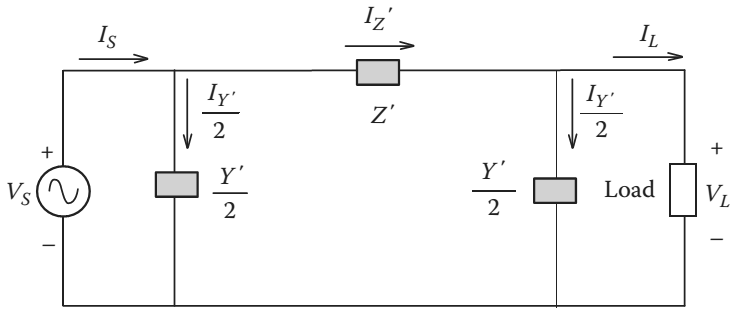
\includegraphics[scale=0.4]{piequi.png}
\caption{Equivalent $\pi$ circuit model of a long-length transmission line}
\end{center}
\end{figure}
\par A high voltage line can be approximated as a lossless line for transmission capacity studies. For such a line, the voltage (V) and current (I) at distance $x$ from the sending end can be determined as follows:
\begin{equation}\label{eqn:abcd}
\begin{bmatrix}
V_x\\
I_x
\end{bmatrix}
=
\begin{bmatrix}
cos(\beta x) & -jZ_c sin(\beta x)\\
-jsin(\beta x)/Z_c & cos(\beta x)
\end{bmatrix}
\begin{bmatrix}
V_s\\
I_s
\end{bmatrix}
\end{equation}
where subscript s stands for sending end. $Z_c$ is the surge impedance of the line which equals to $\sqrt{L_0/C_0}$, $\beta=2\pi/\lambda$ and $\lambda$ is the wavelength. If $x=\lambda /2$, Equation (\ref{eqn:abcd}) becomes
\begin{equation}
\begin{bmatrix}
V_x\\
I_x
\end{bmatrix}
=
\begin{bmatrix}
-1 & 0\\
0 & -1
\end{bmatrix}
\begin{bmatrix}
V_s\\
I_s
\end{bmatrix}
\end{equation}
\par The above equation implies that there is zero impedance between the sending and receiving end of the line, as if the line did not exist. The line only reverses the phase of the voltage and current. The main drawback of the HWTL scheme at 50Hz (low frequency) is its excessive and fixed length. One solution to this problem is to change the frequency of the carrier voltage. The wavelength, $\lambda$ is related to the carrier frequency $f$ through $\lambda =v/f$, where $v$ is roughly equal to the speed of light. If the frequency is raised, the corresponding half-wavelength length can be shortened.
\par This scheme further proposes to use high-frequency generators to produce a required frequency that leads to a half-wavelength matching the distance between the generator and the receiving end. In this scheme, the generator and the line are designed and constructed as one unit that just works for the required transmission distance.
\par The proposed scheme is not intended for networked operation. Its primary goal is to bring a large remote generating plant closer to a load center or a regional network using the HWTL. For example, a nuclear plant can be built at a remote location for safety purposes. But the plant is located at the load center electrically using a HWTL, as the line impedance is close to zero between the generator and the receiving end. According to the relationship between the generator speed ($N_s$) and the pole number ($P$), $f=N_s \times P / 120$ , sample combinations of Ns and P to produce various half-wavelength is shown in Table \ref{tab:pns}. The isolated generation can be at any speed and frequency not only those in Table \ref{tab:pns}; thus, the transmission distance is quite flexible for the proposed HFHW scheme.
\begin{table}[h]
\label{tab:pns}
\begin{tabu} to \textwidth {|X[c]|X[c]|X[c]|X[c]|}
\hline
Pole & Ns = 3600rpm & Ns = 7200rpm & Ns = 14400rpm\\
\hline
P = 2 & 2500km(60Hz) & 1250km(120Hz) & 625km(240Hz)\\
P = 6 & 833km(180Hz) & 417km(360Hz) & 208km(720Hz)\\
P = 12 & 417km(360Hz) & 208km(720Hz) & 104km(1440Hz)\\
\hline
\end{tabu}
\caption{HWTL length with different pole no. ($P$) and generator speed ($N_s$)}
\end{table}
\par The proposed scheme needs only one frequency changer or converter station at the receiving end. Since there is only one frequency changer needed, the scheme becomes attractive in comparison with the HVDC scheme.
\chapter{MAJOR COMPONENTS}
\par The single line diagram of the proposed scheme is shown in Fig \ref{fig:sld}. There are mainly four major components: generator, transformer, transmission line and frequency changer.Preliminary technical feasibility analysis is carried out for the proposed scheme, especially for its four major components below:
\begin{figure}[h]
\label{fig:sld}
\begin{center}
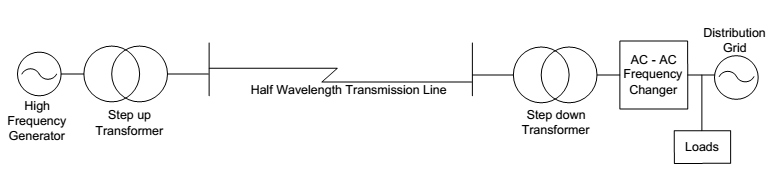
\includegraphics[scale=0.5]{SingleLineDiagram.png}
\caption{HFHW Transmission Single Line Diagram}
\end{center}
\end{figure}
\section{High Frequency Generator}
\par The rotation speed of industrial steam turbine is quite flexible and can be as high as 20000 rpm. For example, steam turbine SST-600 produced by Siemens has a speed range varying from 3000 to 18000 rpm, and has been widely used for power generation. Hence, high frequency power generation is easy to implement.
\par In fact, running a turbine at a higher speed has two additional benefits: 
\begin{itemize}
\item Higher efficiency and lower cost: Each steam turbine has its optimum rotation speed where the efficiency is the highest. Normally, this speed is higher than the generator's speed. Existing solution to deal with this problem is to use gearbox, which causes extra energy loss and requires cooling system. The proposed transmission scheme can increase the generator speed and hence the efficiency could be optimized without using gearbox.
\item Space-saving: The power developed at the turbine shaft is a function of the torque developed at the turbine blades and its rotation speed ($P=\tau\omega$). If the turbine speed is increased, then a smaller diameter turbine would be required to maintain the same power, thus reducing the cost and size.
\end{itemize}
\par As for a hydro power unit, its rotation speed can also be increased through hydraulic design. Increasing the number of poles may not be an option since hydro generators have many poles already.
\section{Transformer \& Transmission Line}
\par Two custom-made high frequency transformers are needed for the scheme; one at the sending end and other at the receiving end. At higher frequencies, a transformer can be made with smaller size and weight for the same power level. The high voltage transformers are always custom made even at 50Hz. So the proposed scheme does not add more work for transformer procurement.
\par The proposed HFHW scheme operates up to roughly a few hundred hertz such as 180Hz to 360Hz shown in Table \ref{tab:pns}. At these frequencies, the technical issues facing a transmission line are similar to those of the 50Hz line. The losses may be higher due to the increased resistance at a higher frequency like skin effect. It might be possible to design conductors with larger equivalent surface area to alleviate the skin effect. Operating at much higher frequencies is also possible but it is not clear at this stage if new technical problems may appear.
\section{Frequency Changer}
\par Frequency changer is the key equipment of the proposed scheme. The frequency conversion can be realized by single-stage AC-AC conversion or two-stage AC-DC-AC conversion. Single-stage AC-AC conversion can achieve higher efficiency while the two-stage conversion with DC-link is more flexible in control and thus could enable more features to improve output quality and system reliability. For two-stage AC-DC-AC converters, the front end can be active or passive rectifiers and the output stage can be either current source converter (CSC) or voltage source converter (VSC). With the half-wavelength line, the generator is "located" electrically at the frequency changer site. Therefore, reactive power compensation is not required and power factor can be controlled to be close to unity using simple generator control. As a result, passive rectifier with diodes or multiple-pulse diode can help to reduce the cost of the frequency changer significantly in comparison with the HVDC converter. Fig. \ref{fig:cyclo} shows an example two-stage AC-DC-AC converter system with 12-pulse diode rectifier at the front end that could be used for the proposed HFHW scheme. It is important to note that the proposed HFHW scheme needs only one converter station at the receiving end. In comparison, two converter stations, one at the sending and another at the receiving end, are needed for the HVDC scheme.
\begin{figure}[h]
\label{fig:cyclo}
\begin{center}
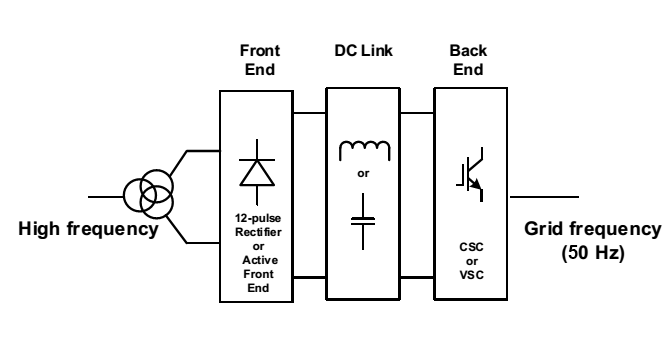
\includegraphics[scale=0.5]{cyclo.png}
\caption{Example Topology of AC-DC-AC Converter for the Proposed HFHW Scheme}
\end{center}
\end{figure}
\par As the field of power electronics is advancing rapidly, many new frequency changers and variable frequency drive schemes are being proposed. Unlike the industrial variable frequency drives, the proposed HFHW scheme only requires to convert from one fixed frequency to another fixed frequency. So there are opportunities to create novel frequency changers that serve this specific need at a much lower cost.
\subsection{Topology}
\par Many proven topologies from high power drives and HVDC industries can be considered for designing the frequency changer. For single-stage AC-AC converter system, the naturally commutated cycloconverter is probably the most economic option at present, due to its simple structure and single-stage conversion. Particularly it fits very well for large-power, frequency step-down applications. Cycloconverter can be constructed by thyristor. Therefore, the successful series-connect application of thyristor in the HVDC system benefits the high voltage/high power application for cycloconverter, making it capable of connecting to high voltage transmission lines. Moreover, the construction, operation and maintenance experiences in high power drive system can also be applied to cycloconverter based HFHW scheme. The annual cost of one cycloconverter based station is estimated to be only 1/3 of two line-commutated converter (LCC) HVDC stations. For a relatively large change of frequency as required in the proposed scheme, the cost of cycloconverter could be slightly higher than 1/3. Such type of cost data is not available yet. Besides, the other AC-AC topologies like matrix converter and other novel AC-AC topologies with lower cost could be considered as well.
\par As mentioned earlier, a unique feature of the proposed HFHW scheme is that diode front end can be used for the two-stage converter system. In this case, the diode rectifier requires series-connect technology to bear the high voltage stress, but the cost is much lower than active rectifiers (like thyristor-based rectifiers or other multilevel converters). For the rear end, many options can be employed. Thyristor-based LCCs, for example, have been widely used in HVDC transmissions. Along with the diode front end, it will be a very cost-effective scheme. Modular Multilevel Converter (MMC) is also a good candidate, boasting its modular structure and capability of operating under high voltage with low voltage components. The modular structure makes MMC easy to maintain with high reliability. Since the output frequency is fixed at grid frequency in this application, MMC will not suffer from the severe capacitor voltage fluctuation under low fundamental frequency. Cascaded H-bridge (CHB) converter is another VSC based topology that can be applied. This topology suits very well for multi-pulse diode front end with multi-winding isolation transformer. As VSCs with DC-link, MMC and CHB are capable of injecting reactive power and interfacing weak grid. These advantages make them attractive even considering their relatively high cost. Beside the existing proven topologies, the HFHW scheme also offers a new motive for developing novel AC/AC and multilevel converter topologies.
\subsection{Devices}
\par Diodes, thyristors and IGBTs are all widely used and their power ratings are continuously increasing while the prices are falling. In general, the price of a single IGBT module with its gate driver rises significantly as the power rating goes up, thus thyristor based or diode based converters have advantages on cost in high power applications, especially the diodes. However, IGBT based VSC converters are 50-60\% more compact than thyristor based ones, leading to smaller converter stations size and thus the overall cost of VSC converter stations is only 10-15\% higher comparing to LCC stations.
\par Meanwhile, next generation power switches - wide band-gap devices, such as SiC MOSFETs or IGBTs, make it possible to further increase the rated voltage of semiconductor devices. Although some multilevel converters can realize high voltage application with low voltage semiconductor devices, developing high voltage high frequency devices is still helpful to simplify the system structure and thus increase the reliability. Considering the large power that flowing through the converters, efficiency is another important concern, which can also be improved by applying wide band-gap devices. The main disadvantage of these devices at the moment is the cost. However, as wide band-gap devices tend to be more adopted applied, the cost is becoming more acceptable considering the benefits they bring. Therefore, further improvements on reliability and efficiency of the frequency changer are very possible. This will benefit the proposed HFHW scheme as well as the HVDC scheme.
\subsection{Control Strategies}
\par Power electronic equipment will handle the high power flow like in a HVDC system, instead of working as an auxiliary apparatus like active power filter (APF) and STATCOM. Thus, reliability will be very important for the frequency changer. Specifically for the proposed scheme, the frequency changer's main task is to deliver the power generated by the remote generator to the load center. Therefore, proper power flow control using the frequency changer will be required. In case the load center is not connected to a stiff power frequency grid, control the load center voltage (magnitude and frequency) and maintain superior power quality would be necessary. Additionally, although reactive power from the front end is not needed due to the fact that the generator can control reactive power, reactive power can be easily produced from the back end converter to support the load center. Finally, the control strategies that enable the frequency changer to operate under harmonic distortion, grid faults (symmetrical or unbalanced), and component failure are key for operating such the HFHW system.
\chapter{TRANSMISSION CHARACTERISTICS}
This section presents a basic analysis on the voltage profile and transmission capability of the proposed HFHW scheme. The data of typical transmission line is shown in Table \ref{tab:tl}. If we normalize the data using the rated voltage and surge impedance loading (SIL) level of the respective lines as the base values, all transmission lines have the same per-unit reactance and admittance values (the last row of Table \ref{tab:tl}). The per-unit values are used to conduct analysis.
\begin{table}[h]
\label{tab:tl}
\begin{tabu} to \textwidth {|X[c]|X[c]|X[c]|X[c]|X[c]|X[c]|}
\hline
Voltage & R ($\Omega$/km) & X ($\Omega$/km) & B ($\mu S$/km) & $Z_{surge}$ ($\Omega$) & SIL (MW)\\
\hline
138kV & 0.2140 & 0.4801 & 3.4321 & 374 & 51\\
240kV & 0.0626 & 0.3681 & 4.4936 & 286 & 201\\
345kV & 0.0370 & 0.3670 & 4.5180 & 285 & 418\\
500kV & 0.0280 & 0.3250 & 5.2000 & 250 & 1000\\
per unit & vary & 0.00126 & 0.00126 & 1 & 1\\
\hline
\end{tabu}
\caption{Typical Transmission Line Data}
\end{table}
\section{Voltage Profile}
\par The voltage profile of a 500kV, 180Hz HWTL is shown in Fig. \ref{fig:lossless} and Fig. \ref{fig:lossy}. Fig. \ref{fig:lossless} shows the lossless line and Fig. \ref{fig:lossy} includes line losses (0.028 $\Omega$/km). The voltage profiles of the line under other frequencies are similar. The length of the HWTL is 190 electric degree, rather than the exact 180 electric degree ($\lambda /2^+$ Transmission). The reasons are:
\begin{itemize}
\item To reduce the required sensitivity of the generator reactive power output control
\item To assure having a full half-wavelength during the frequency variation
\end{itemize}
\par The results reveal the following unique characteristic of the proposed HFHW scheme: the voltage profile exhibits a large change along the line. It rises at the middle point of the line. The degree of change is in proportion to the line loading level (in the form of multiple of SIL level). A higher loading level results in higher voltage at the middle point.
\begin{figure}[h]
\label{fig:lossless}
\begin{center} 
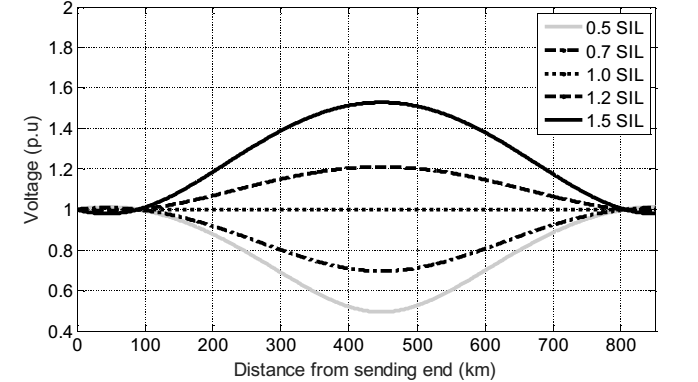
\includegraphics[scale=0.5]{lossless.png}
\caption{Voltage Distribution of Lossless HWTL}
\end{center}
\end{figure}
\begin{figure}[h]
\label{fig:lossy}
\begin{center}
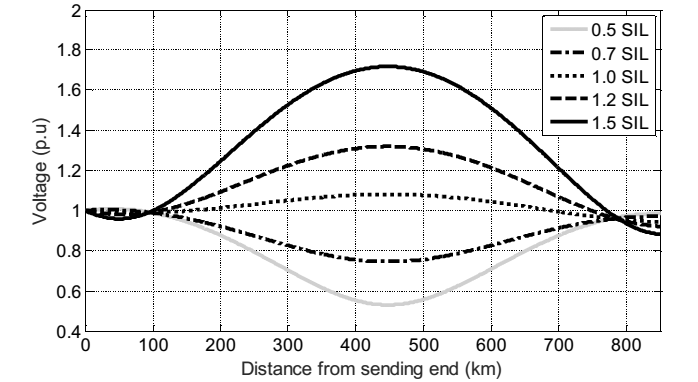
\includegraphics[scale=0.5]{lossy.png}
\caption{Voltage Distribution of Lossy HWTL}
\end{center}
\end{figure}
\section{Power Transfer Capability}
\par The power transfer capability of traditional transmission lines is constrained by voltage stability, angular stability and conductor thermal limits. Since the impedance of such lines increase with the transmission distance, the maximum power that can be transmitted will decrease. The relationship between the maximum transferable power versus transmission distance is described as the St. Clare curve.
\par The transmission power limit is given by,
\begin{equation}\label{eqn:pmax}
P_{max}=\frac{V_sV_r}{Z_csin\beta l}=\frac{P_n}{sin\beta l}
\end{equation}
where $V_s$ and $V_r$ are voltages at sending and receiving ends of transmission line respectively; $Z_c$  is characteristic
impedance, $\beta$ is phase constant and $P_n$ is natural power.
\par As it is seen from the equation \ref{eqn:pmax}, when $\beta l=\pi$ , the transmission power limit is the natural power and when $\beta l=\pi/2$, the electrical distance equals to the half-wave length, transmission power will rise to infinity in the ideal condition, but the actual transmission power is usually subject to the voltage distribution along the line, line insulation level and other factors.
\begin{figure}[h]
\label{fig:transcap}
\begin{center}
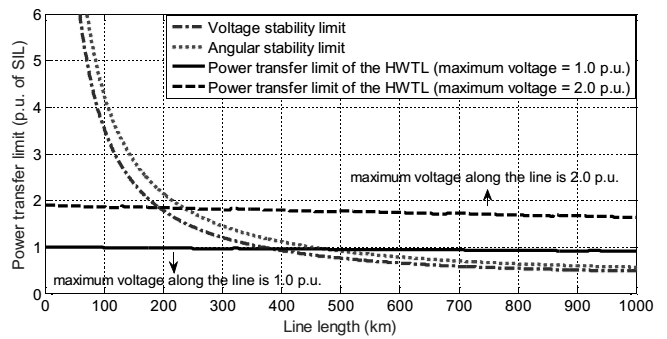
\includegraphics[scale=0.6]{transcap.png}
\caption{Transmission Capability Curves of Lossy Transmission Lines}
\end{center}
\end{figure}
\par Fig. \ref{fig:transcap} shows the comparison of the power transfer limits as a function of the transmission distance. Since the HWTL line has very small impedance between the sending and receiving ends, its transmission capability is essentially not constrained by the stability limits, i.e. the transmission distance. Its maximal power transfer capability is determined by the voltage level at the middle point. For example, if one allows the voltage rises to twice of the rated voltage by design, around 2$\times$SIL power can be transmitted regardless of the transmission distance. Since the proposed scheme does not have a 1.0 pu voltage profile, the current at two ends can be large. The conductor size and sag could be another design limit to consider if the high rated voltage can be adopted.
\chapter{MULTITERMINAL TRANSMISSION}
\par The proposed HVAC tap is based on the power-electronics converters and provides a multiterminal bidirectional power flow capability to the $\lambda /2^+$ transmission system. The HVAC tap can be used to connect local systems, generation, and loads, to a $\lambda /2^+$ transmission line.
\par The electrical behavior of a $\lambda /2^+$ line with an HVAC tap depends of the connection type and the tap position along the line. The HVAC tap can be an HVAC series tap or an HVAC shunt tap. This chapter evaluates the main effects of an HVAC tap connected to a $\lambda /2^+$ line. The evaluation is in terms of: 
\begin{itemize}
\item Transmitted power and reactive power
\item Voltage profile.
\end{itemize}
\section{Series Tap}
\begin{figure}[h]
\label{fig:seriestapckt}
\begin{center}
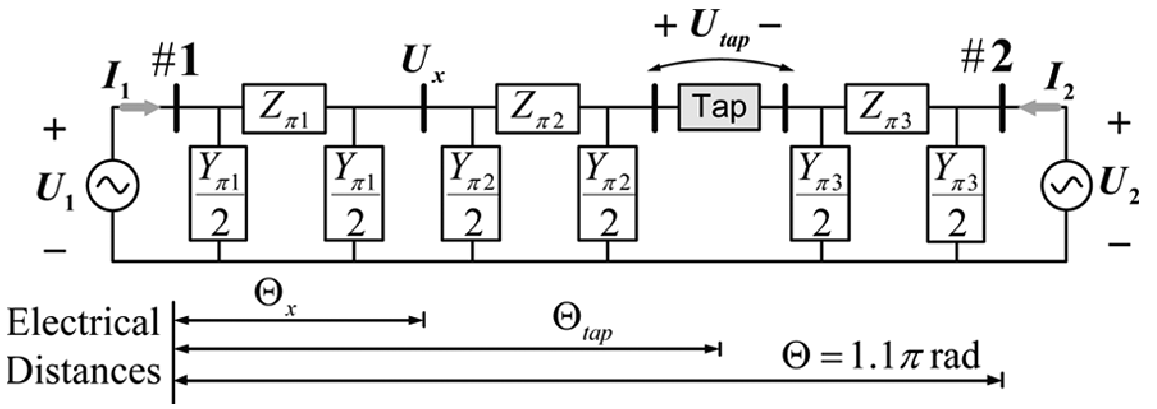
\includegraphics[scale=0.3]{seriestapckt.png}
\caption{Equivalent circuit for the analysis of the HW system with a series tap, for $\Theta_{tap} > \Theta_x $ }
\end{center}
\end{figure}
\par Fig. \ref{fig:seriestapckt} shows two large power systems, represented as infinite buses, tied by a $\lambda /2^+$ line. An HVAC series tap is connected to the line at an equivalent electrical distance from bus \# 1. The $\lambda /2^+$ line is assumed ideal and is divided into three sections which are represented as the equivalent- model, and the terminal voltages are $U_1 = 1.0\angle \delta pu$ and $U_2 = 1.0\angle 0 pu$, with $\delta = 1.1\pi rad$. The equivalent electrical length of each $\pi$-section is varied to calculate the voltage at different points along the line $\Theta_x$ for a different tap position $\Theta_{tap}$.
\begin{figure}[h]
\label{fig:seriestappower}
\begin{center}
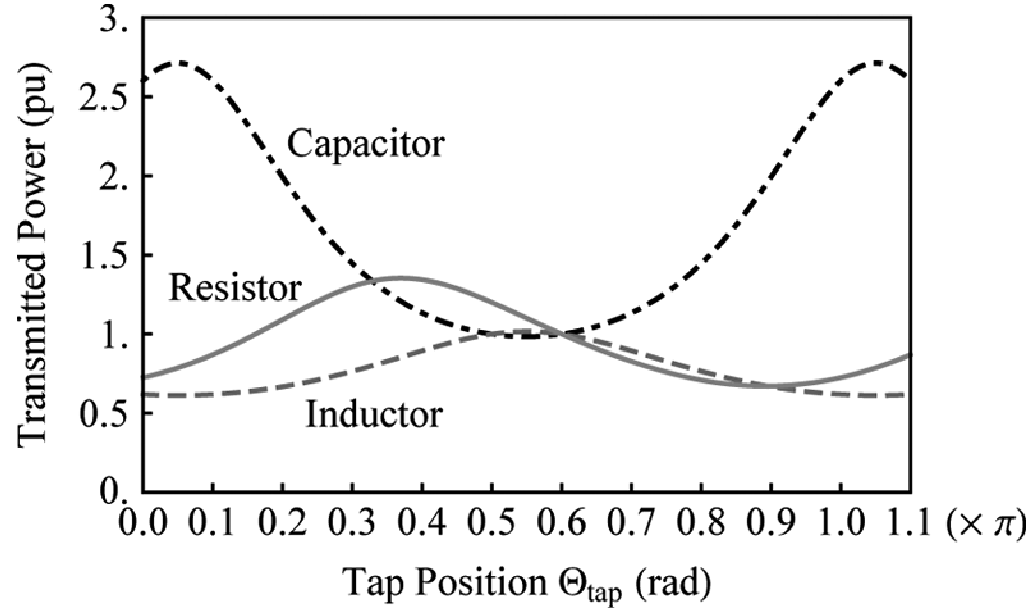
\includegraphics[scale=0.3]{seriestappower.png}
\caption{Transmitted power as a function of the series tap’s impedance and position.}
\end{center}
\end{figure}
\begin{figure}[h]
\label{fig:seriestaprepower}
\begin{center}
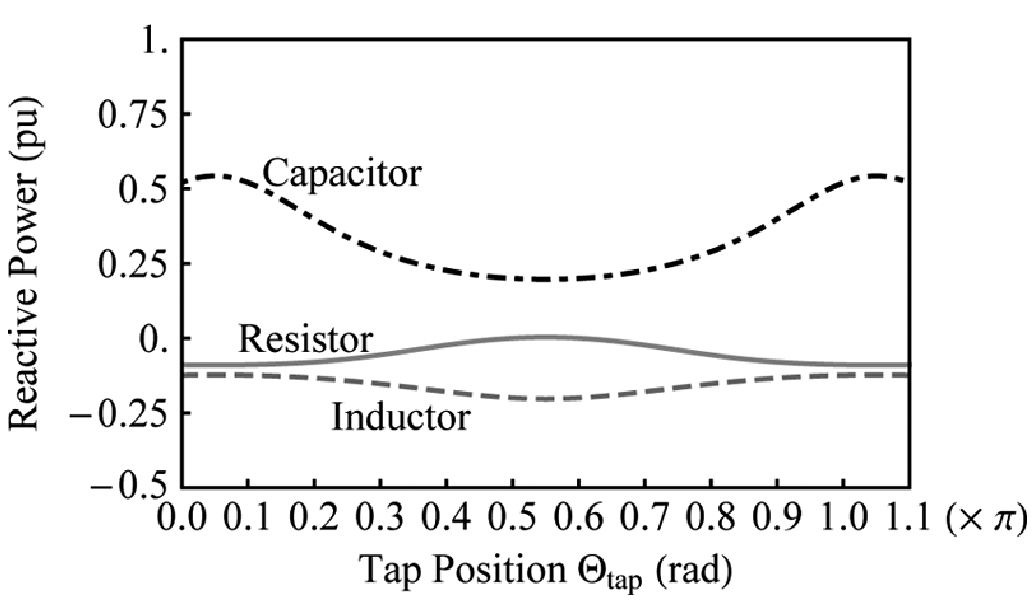
\includegraphics[scale=0.3]{seriestaprepower.png}
\caption{Reactive power as a function of the series tap’s impedance and position.}
\end{center}
\end{figure}
\par Fig. \ref{fig:seriestappower} shows the transmitted power at bus \# 1 for a 0.2 p.u. series tap connected to the $\lambda /2^+$ line. The tap is modeled as a passive load (i.e., a resistor, a capacitor, or an inductor).
\par Fig. \ref{fig:seriestappower} indicates that the transmitted power is more sensitive to series loads connected near the terminals than to series loads connected around the central region of the line. For instance, a 0.2 p.u. series capacitor connected to the bus \# 1 can increase the transmitted power from 1.0 to 2.5 p.u..Fig. \ref{fig:seriestaprepower} shows that the line reactive power is less affected than the transmitted power for a series load in the line. For active power draining (i.e., for a pure series resistor), Fig. \ref{fig:seriestappower} and Fig. \ref{fig:seriestaprepower} indicate that an HVAC series tap does not significantly affect the transmitted power and reactive power, if it is connected around the central region.
\begin{figure}[h]
\label{fig:seriestapvpdp}
\begin{center}
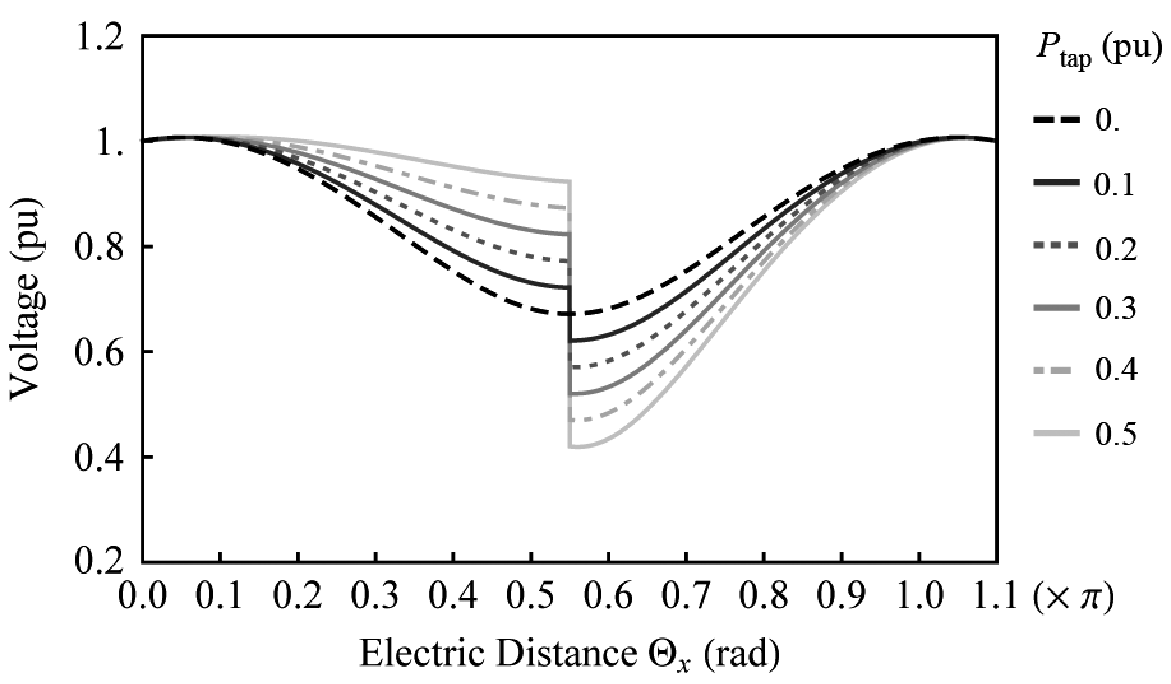
\includegraphics[scale=0.3]{seriestapvpdp.png}
\caption{Voltage profile as a function of the series tap’s drained power, for $\Theta_{tap}=0.5\Theta$.}
\end{center}
\end{figure}
\begin{figure}[H]
\label{fig:seriestapvpip}
\begin{center}
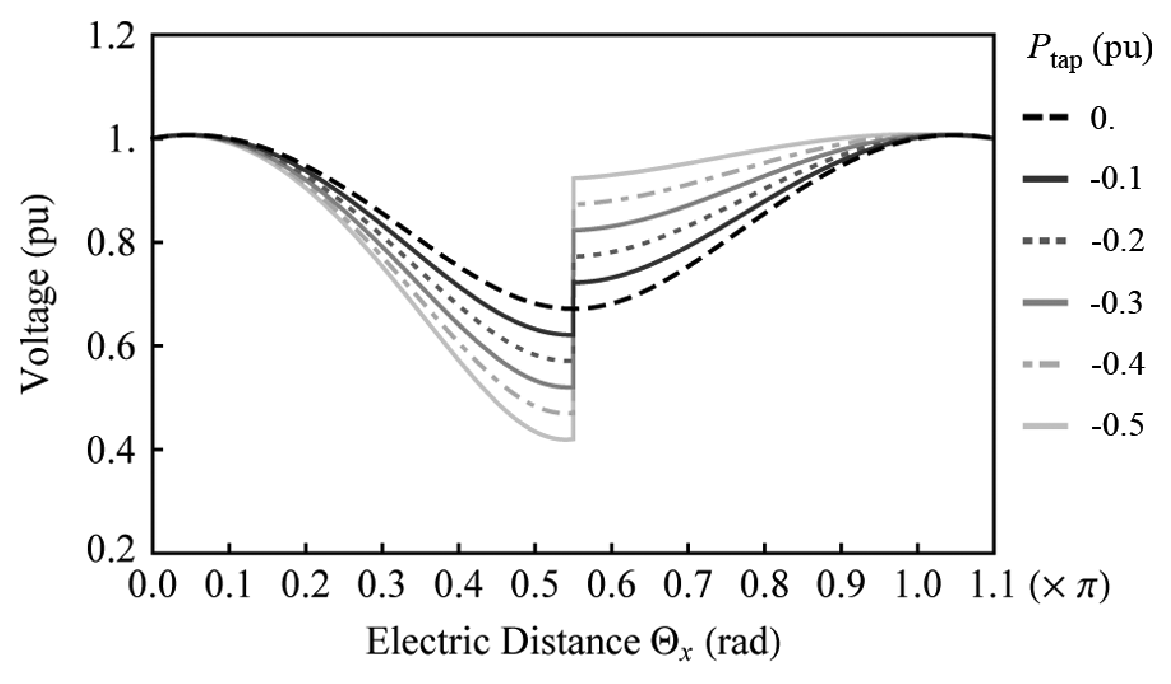
\includegraphics[scale=0.3]{seriestapvpip.png}
\caption{Voltage profile as a function of the series tap’s injected power, for $\Theta_{tap}=0.5\Theta$.}
\end{center}
\end{figure}
\par For a full loaded $\lambda /2^+$ line (i.e. $\delta = \Theta$), the transmitted power may exceed the limit $|P_1 \leq P_c$, when a resistive series tap is connected along the line, as shown in Fig. \ref{fig:seriestappower}. As a consequence, the voltage along the line may exceed $U_0$. However, if $P_1$ is adjusted to remain lower than $P_c$, the voltage along the line will be lower than $U_0$ even for a series tap connected to the central region. Fig. \ref{fig:seriestapvpdp} and Fig. \ref{fig:seriestapvpip} exhibit the voltage profile for a 97\% loaded line (i.e., $P_1=0.97P_c$ ) as a function of the series power tap $P_{tap}$. In Fig. \ref{fig:seriestapvpdp} and Fig. \ref{fig:seriestapvpip}, $P_{tap}>0$ indicates drained power from the line and $P_{tap}<0$ indicates injected power to the line respectively. It is noticeable that the voltage along the line does not exceed even in the presence of a series tap connected at the line half length.
\par Fig. \ref{fig:seriestaptppa} presents the transmitted power as a function of the power angle for different values of the series tap power drain located at the half length of the $\lambda /2^+$ line. Fig. \ref{fig:seriestaptppa} indicates that if the terminal voltages are kept constant, the transmitted power at the sending end increases proportionally to the drained power by the tap. In terms of a steady-state stability point of view, it is noticeable that the system stability is maintained even in the presence of the series tap, since the power-angle derivative is positive and constant. In summary, this analysis indicates that the HVAC series tap may be a solution to provide multiterminal connection capability to a $\lambda /2^+$ transmission line when it is connected around the central region of the line. Moreover, the HVAC series tap, operating as a FACTS device, may be very effective to control the main power flow when it is connected near the line terminals.
\begin{figure}[h]
\label{fig:seriestaptppa}
\begin{center}
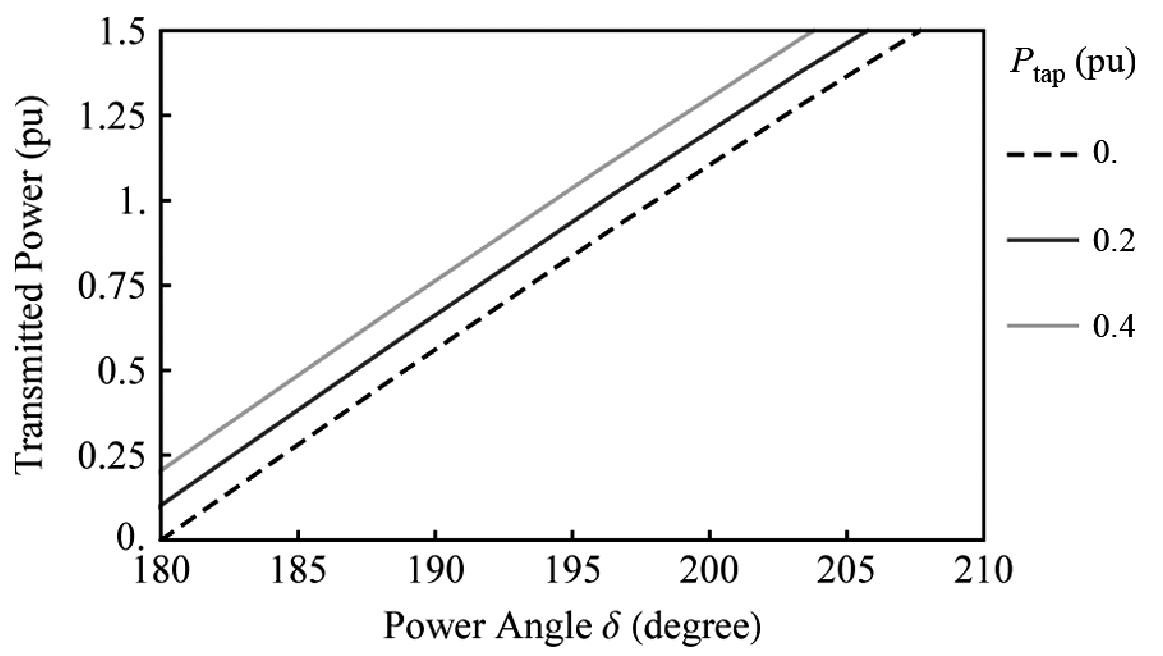
\includegraphics[scale=0.3]{seriestaptppa.png}
\caption{Transmitted power at terminal \#1 as a function of the power angle, for $\Theta_{tap}=0.5\Theta$.}
\end{center}
\end{figure}
\section{Shunt Tap}
\begin{figure}[h]
\label{fig:shunttapckt}
\begin{center}
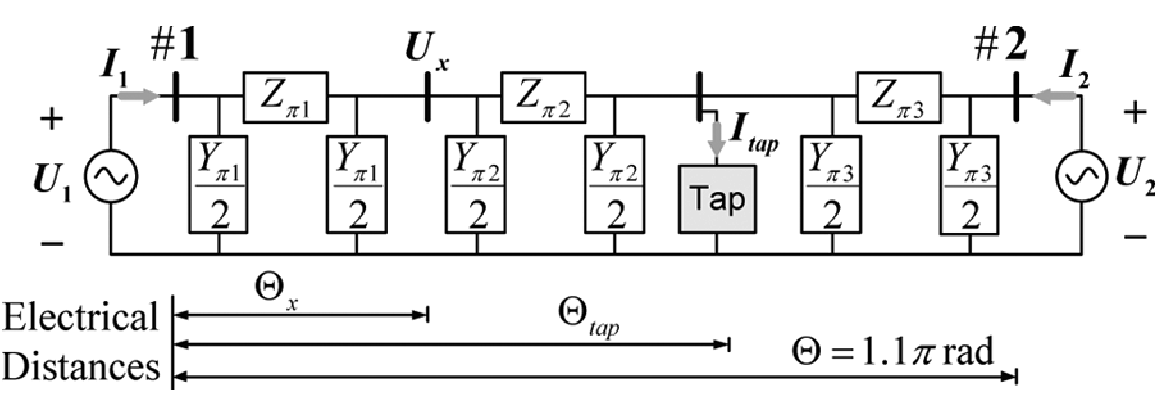
\includegraphics[scale=0.3]{shunttapckt.png}
\caption{Equivalent circuit for the analysis of the HW system with a shunt tap, for $\Theta_{tap} > \Theta_x $ }
\end{center}
\end{figure}
\par Fig. \ref{fig:shunttapckt} shows the single-line diagram used to evaluate the effect of an HVAC shunt tap on a $\lambda /2^+$ line. The power system is the same as that of Fig. \ref{fig:seriestapckt}, and the HVAC tap is connected through an ideal power shunt transformer.
\begin{figure}[h]
\label{fig:shunttappower}
\begin{center}
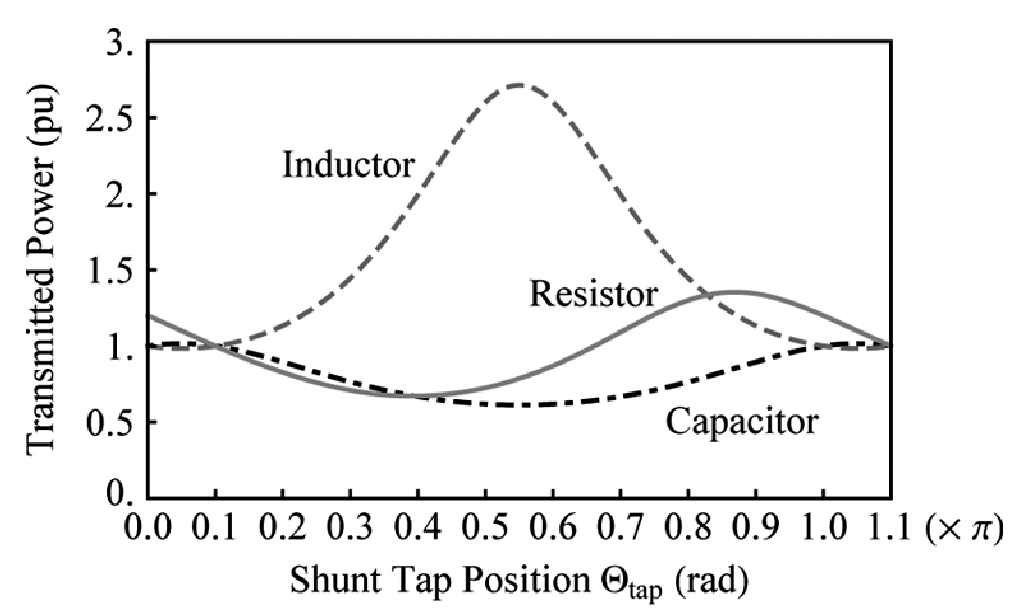
\includegraphics[scale=0.3]{shunttappower.png}
\caption{Transmitted power as a function of the series tap’s impedance and position.}
\end{center}
\end{figure}
\begin{figure}[h]
\label{fig:shunttaprepower}
\begin{center}
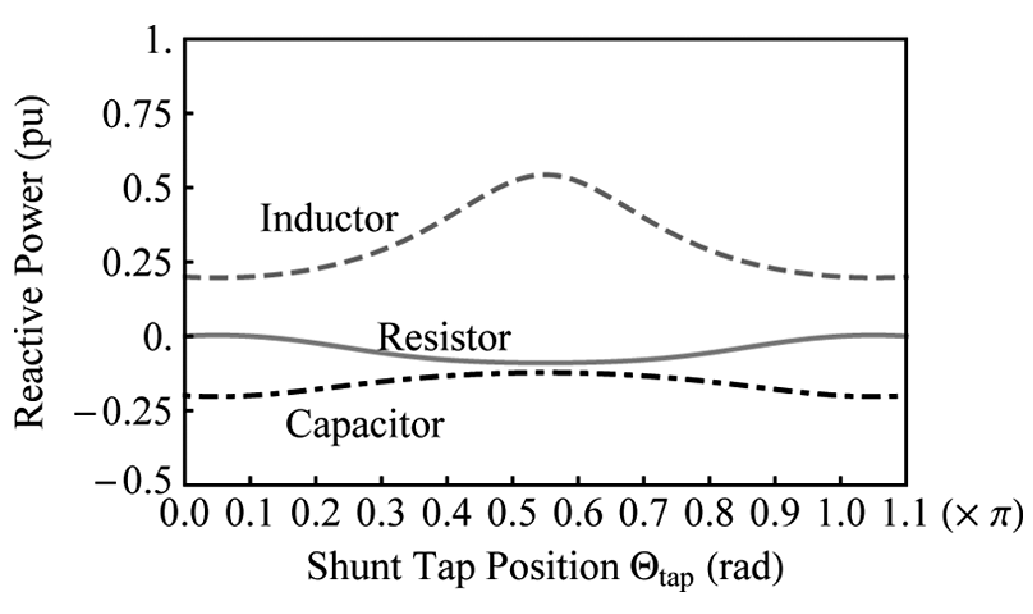
\includegraphics[scale=0.3]{shunttaprepower.png}
\caption{Reactive power as a function of the series tap’s impedance and position.}
\end{center}
\end{figure}
\par Fig. \ref{fig:shunttappower} evaluates the transmitted power through a $\lambda /2^+$ line with a shunt tap as a function of the tap’s position and impedance. Three different impedances are considered, corresponding to a capacitor, a resistor and an inductor. The objective is to show how a load affects the electrical behavior of the line. Fig. \ref{fig:shunttappower} indicates that the transmitted power is less sensitive for reactive loads located near the line terminals. On the other hand, the reactive power is lower for resistive loads in the same regions, as shown in Fig. \ref{fig:shunttaprepower}. The transmitted power is significantly affected by shunt reactive loads connected around the line central region, which indicates that the line power flow might be controlled with shunt FACTS devices in the central region.
\begin{figure}[h]
\label{fig:shunttapvpdp}
\begin{center}
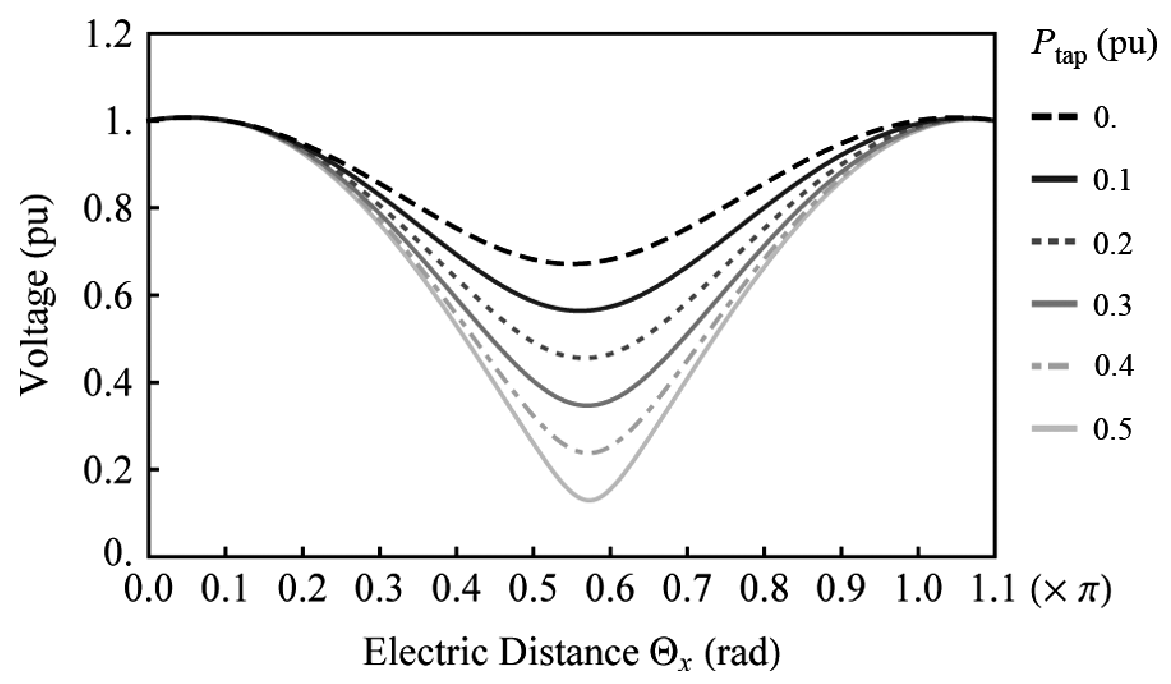
\includegraphics[scale=0.3]{shunttapvpdp.png}
\caption{Voltage profile as a function of the shunt tap’s drained power, for $\Theta_{tap}=0.5\Theta$.}
\end{center}
\end{figure}
\begin{figure}[h]
\label{fig:shunttapvpip}
\begin{center}
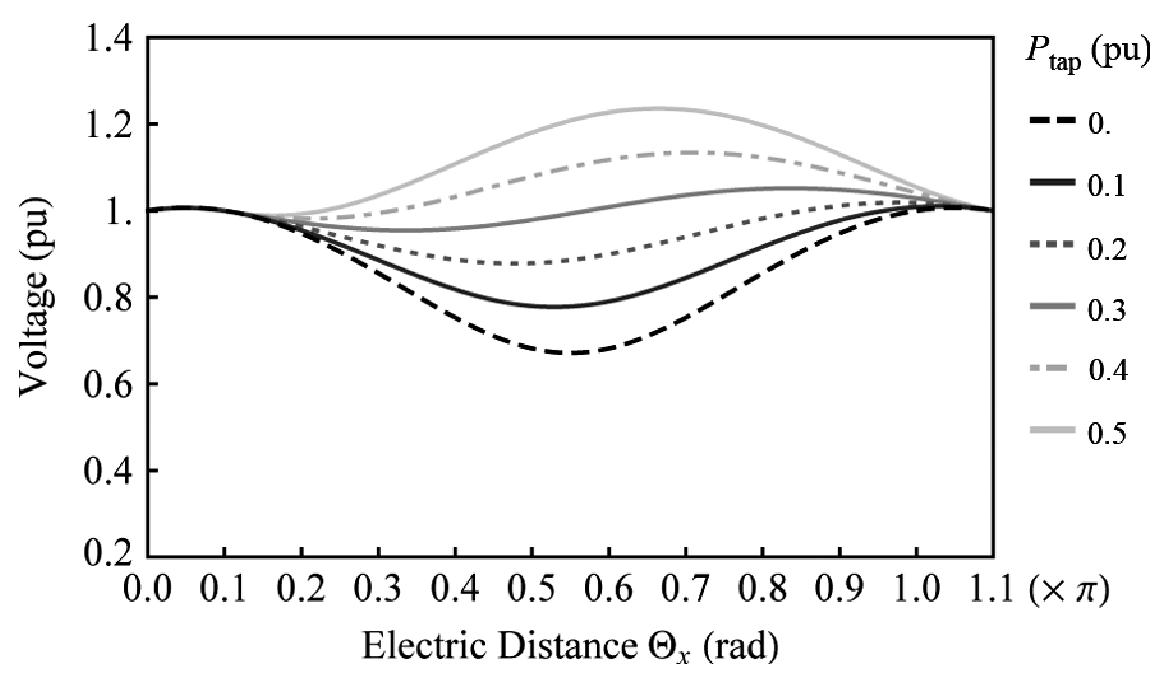
\includegraphics[scale=0.3]{shunttapvpip.png}
\caption{Voltage profile as a function of the shunt tap’s injected power, for $\Theta_{tap}=0.5\Theta$.}
\end{center}
\end{figure}
\par Similar to the series tap, in a full loaded line, the voltage profile may exceed $U_0$ when a shunt tap draining power is connected close to the line terminals. However, the voltage does not exceed if the transmitted power is lower than $P_c$. Fig. \ref{fig:shunttapvpdp} exhibits the voltage profile as a function of for a shunt tap connected close to the line sending end (i.e., at 275 km), when $P_1=0.97P_c$. It is noticeable that the voltage does not exceed $U_0$. On the other hand, when a shunt tap injects power to the $\lambda /2^+$ line at $\Theta_{tap}=0.11\pi rad$, the voltage along the line may exceed if the injected power increases, as shown in Fig. \ref{fig:shunttapvpip}. For a shunt tap connected close to the line receiving-end, an opposite effect is observed (i.e., the voltage along the line may exceed $U_0$ if a large amount of power is drained).
\begin{figure}[H]
\label{fig:shunttaptppa}
\begin{center}
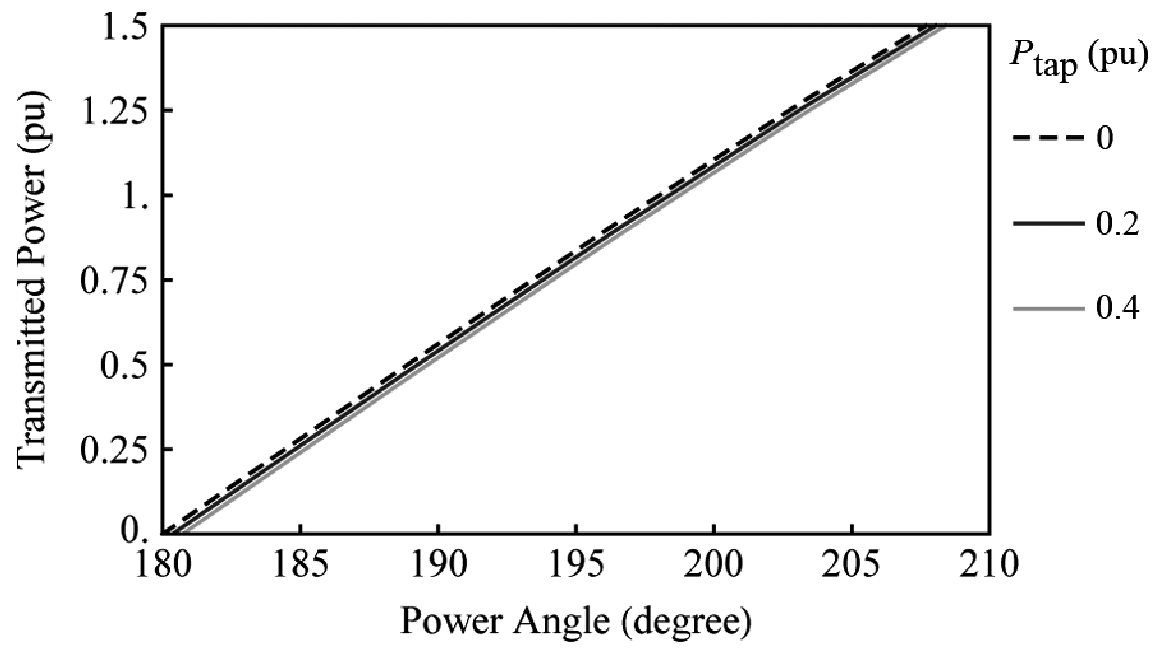
\includegraphics[scale=0.3]{shunttaptppa.png}
\caption{Transmitted power at terminal \#1 as a function of the power angle, for $\Theta_{tap}=0.5\Theta$.}
\end{center}
\end{figure}
\par Fig. \ref{fig:shunttaptppa} shows the effect of a shunt tap on the transmitted power. The shunt tap is closer to the sending-end terminal and different values of drained power are analyzed. Fig. \ref{fig:shunttaptppa} indicates that the transmitted power is barely affected by a shunt tap near to the sending-end which means that shunt tap reduces the power delivered to terminal \#2. The same effect is observed when the shunt tap is injecting power to the line at the same position. In the stability point of view, this results indicate that the shunt tap does not affect system stability, since the power-angle derivative is positive and constant.
\par This analysis concludes that the shunt tap is suitable for power draining/injection close to line terminals. However, the voltage along the line may exceed if the power tap is very high. This drawback is more severe if the line is fully loaded.

\chapter{ADVANTAGES OF HFHW TRANSMISSION}
Compared to conventional AC transmission, half-wavelength transmission technology has some distinct features and advantages as a special type of very long distance AC transmission:\\~\\
\space\space $\bullet$ \textbf{No need to install reactive power compensation equipment along the all line.}\\
In conventional UHV power transmission, reactive power regulation is an important key technical problem. The voltage at terminal end of transmission line with no load increase with line length, in the most adverse conditions, it can be several times higher than the supply voltage. Installing a large number of reactive power compensation devices such as high-voltage reactor is essential. However the voltage variation of HWACT along the transmission line is completely different, we can use the following equation \ref{eqn:vi} to analyze the voltage and current (assuming the line is lossless and line length is exactly half the wave length).
\begin{equation}\label{eqn:vi}
V_r=V_scos(\beta l)-jZ_csin(\beta l)
\end{equation} 
Since $\beta l=\pi$ for half-wavelength line, $|V_r|=|V_s|$. This means that the voltage at both ends of the lossless half-wavelength line remains equal, i.e.,for the line with load or no load, the voltage amplitudes are consistent. Thus there is no need to install reactive compensation equipment.\\~\\
\space\space $\bullet$  \textbf{More Power Transmission Capability.}\\
From Equation \ref{eqn:pmax} we can see, in a standard half-wavelength ($\beta l=\pi$) line, the theoretical maximum transmission capacity can be up to infinity. Analysis showed that taking over-voltage limits, line capacity, corona loss and other factors into account, the maximum transmission capacity of 3000 km half-wavelength transmission is up to 1.0 - 1.2 times of the natural power.\\~\\
\space\space $\bullet$ \textbf{No need to construct intermediate switching station.}\\
For long distance conventional UHV AC transmission, due to the stability margin and for reactive power compensation, it is needed to cut the transmission line into segments and to construct switching stations; While in half-wave length transmission technology, since there is no need for reactive power compensation and has good power transmission capability, it does not require intermediate switching station to achieve point to point transmission as HVDC transmission.\\~\\
\space\space $\bullet$ \textbf{Absence of Ferranti Effect.}\\
The Ferranti effect is an increase in voltage occurring at the receiving end of a long transmission line, above the voltage at the sending end. This occurs when the line is energized, but there is a very light load or the load is disconnected. The capacitive line charging current produces a voltage drop across the line inductance that is in-phase with the sending end voltages considering the line resistance as negligible. Therefore both line inductance and capacitance are responsible for this phenomenon. The Ferranti Effect will be more pronounced the longer the line and the higher the voltage applied. The relative voltage rise is proportional to the square of the line length. There is no such problem in HFHW transmission.\\~\\
\space\space $\bullet$ \textbf{Slightly higher reliability compared to HVDC transmission.}\\
HFHW system and HVDC transmission system has almost the same level in reliability. The quantitative evaluation shows that HFHW has a little higher level in reliability than HVDC.\\~\\
\space\space $\bullet$ \textbf{Less converter station losses to cost ratio compared to HVDC.}\\
Considering the converter station losses, $\pm$800 kV HVDC has a higher loss rate than that of HFHW and the construction cost is also higher. The loss rate of $\pm$1000 kV HVDC is lower, but the construction cost is too high. Though the single-circuit transmission line of HFHW has a lower capacity than HVDC, HFHW has a great advantage in construction cost. So it has a higher economic level than that of $\pm$800 kV HVDC and $\pm$1000 kV HVDC.
\chapter{RESEARCH NEEDS AND ECONOMICS}
\par The proposed HFHW scheme offers a unique advantage for power transmission, namely, "locating" a remote generator electrically at the load center. It thereby overcomes the number one challenge of transmitting power over long distances. However, the scheme exhibits considerably different voltage and current characteristics in comparison with the traditional transmission lines. These characteristics could be a challenge for its implementation, but they may also represent opportunities for further cost savings.
\par For example, the varying voltage profiles of the line may lead to designing a transmission line that has a few different voltage and current ratings along the line. In addition, the proposed scheme could also promote the research in high-frequency generators, high-frequency transformers, and HFHW based frequency changers.According to certain analysis, the major factor making the HWTL costly is its line cost including capital and operating costs. Therefore, the HVDC scheme has clear advantages for long-distance transmission. The proposed HFHW scheme has a shorter distance. In addition, it does not encounter stability constraints so a line with lower voltage rating could be used. These two factors can make the line cost more competitive for the proposed scheme. However, the scheme requires a frequency changer. Since the frequency changer works on a fixed frequency and there is little requirement on control capability, its cost can be attractive in comparison with that of the HVDC converter (especially considering single converter station requirement in the proposed scheme in comparison with the two converter station requirement in the HVDC scheme). Taking into account of all these factors, there is a range of distance where the HFHW scheme could be attractive economically in comparison with the HVDC scheme. A very rough estimate of the break-even distance is about 1000km. Note that this estimate is for the purpose of presenting a rough idea on the potential cost. It is not to declare the cost competitiveness of the proposed method.
\par In summary, the main competitor of the proposed HFHW scheme is the HVDC transmission scheme. It is worthwhile to note that the economics of the HVDC scheme were not attractive either when the scheme was conceived. It has taken more than 50 years effect to make the scheme a technology with industry acceptance. The proposed scheme is in its infancy and it needs time and effort to grow. The main characteristic of the scheme, almost zero electrical distance between the sending and receiving ends regardless of the physical distance, is so technically unique and appealing. Through persistent research, the scheme may find some interesting applications unforeseeable today.
\chapter{CONCLUSION}
\par A new transmission scheme, high frequency power generation and half-wavelength transmission in one unit, is presented. The scheme is not affected by the distance between the generator and load center: it operates as if there is no electrical distance between the sending and receiving end even through the actual physical distance is large. Preliminary feasibility analysis indicates that the scheme is highly feasible technically. It has additional advantages such as improving the efficiency of generators. The proposed scheme also opens opportunities for power electronics, as frequency changer is a key component in the system. It is hoped that this scheme will serve as a step stone in creating innovative power transmission and power electronics technologies for the future power systems.
%-----------------------------------------------------%

\newpage
\newgeometry{top=1.5in}
\pagenumbering{gobble}%Turn off page numbering
%%%%%%References%%%%%%
\thispagestyle{empty}%Turn off header and footer
\begin{center}
\begin{large}
\textbf{REFERENCES}
\end{large}
\end{center}
\addcontentsline{toc}{section}{\bibname}
\begin{thebibliography}{}
\bibitem{}Yang Wang, Wilsun Xu, Yun Wei Li and Tian Hao \emph{"High-Frequency, Half-Wavelength Power Transmission Scheme"}, IEEE Transactions on Power Delivery, July 2016.
\bibitem{}F. J. Hubert and M. R. Gent, \emph{"Half-wavelength power transmission lines"}, IEEE Transactions on Power Apparatus and Systems, vol. 84, no. 10, pp.965-974, Oct. 1965.
\bibitem{}R. Dias, A. Lima, C. Portela, and M. Aredes, \emph{"Extra long-distance bulk power transmission"}, IEEE Trans. Power Del., vol. 26, no. 3, pp.1440–1448, Jul. 2011.
\bibitem{}Y. Song, B. Fan, Y. Bai, X. Qin, and Z. Zhang, \emph{"Reliability and economic analysis of UHV half-wave-length AC transmission"}, Proceedings of 2012 IEEE POWERCON, Oct. 30 - Nov. 2, 2012, pp.1-6.
\bibitem{}M. L. Santos, J. A. Jardini, R. P. Casolari, R. L. Vasquez-Arnez, G. Y. Saiki, T. Sousa, and G. L. C. Nicola, \emph{"Power transmission over long distances: economic comparison between HVDC and half-wavelength line"}, IEEE Trans. Power Del., vol. 29, no. 2, pp. 502-509, Feb. 2014.
\bibitem{}F. S. Prabhakara, K. Parthasarathy and H. N. R. Rao, \emph{"Performance of tuned half-wave-length power transmission lines"}, IEEE Transactions on Power Apparatus and Systems, vol. 88, no. 12, pp. 1795-1802, Dec. 1969.
\bibitem{}F. Z. Peng, L. Chen, and F. Zhang, \emph{"Simple topologies of PWM AC–AC converters"}, IEEE Power Electronics Letters, vol. 1, no. 1, pp. 10–13, Mar. 2003.
\bibitem{}J. W. Kolar, T. Friedli, J. Rodriguez and P. W. Wheeler, \emph{"Review of three-phase PWM AC–AC converter topologies"}, IEEE Transactions on Industrial Electronics, vol. 58, no. 11, pp. 4988-5006, Nov. 2011.
\end{thebibliography}
%-----------------------------------------------------%
\end{document}
%----------------------END----------------------------%